% diag_threat_model: TikZ twin of paper/figures/diag_threat_model.pdf (generated by diag_common.py).
% Coordinates are inches (y up). Needs \usepackage{tikz}. Body font 7 pt.
\definecolor{dgA}{HTML}{F0F0F0}\definecolor{dgB}{HTML}{DCDCDC}\definecolor{dgC}{HTML}{C4C4C4}
\definecolor{dgAtk}{HTML}{F2C9B8}\definecolor{dgHw}{HTML}{E3EEF7}
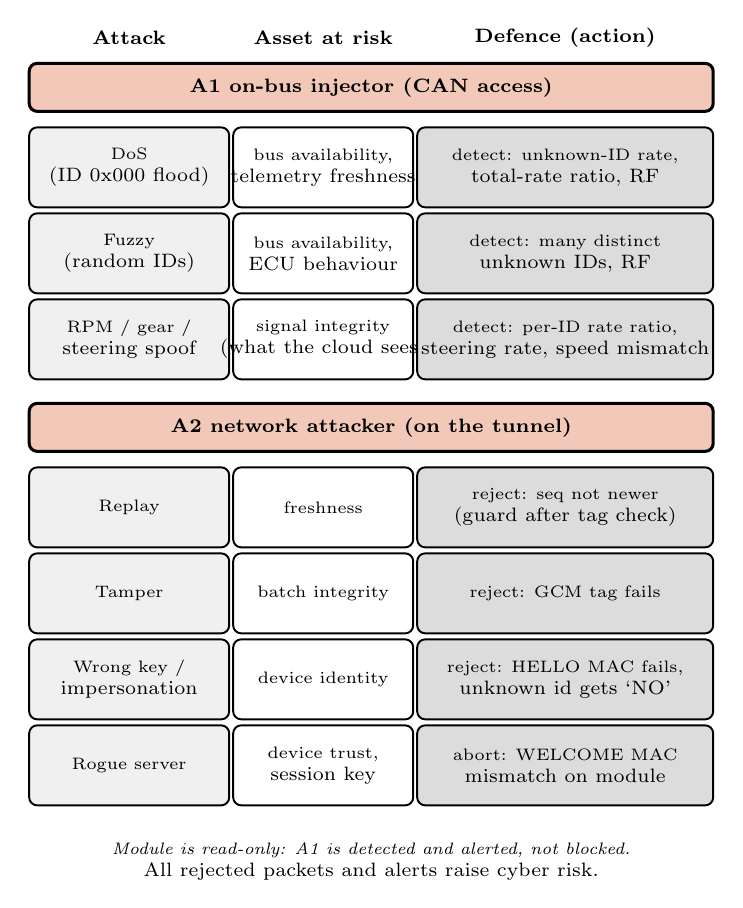
\begin{tikzpicture}[x=1in,y=1in,>=stealth,font=\fontsize{7}{8}\selectfont,line width=0.7pt]
\node[align=center,inner sep=0pt] at (0.540,4.320) {\bfseries \fontsize{6.8}{7.6}\selectfont Attack};
\node[align=center,inner sep=0pt] at (1.510,4.320) {\bfseries \fontsize{6.8}{7.6}\selectfont Asset at risk};
\node[align=center,inner sep=0pt] at (2.720,4.320) {\bfseries \fontsize{6.8}{7.6}\selectfont Defence (action)};
\draw[rounded corners=2.9pt,fill=dgAtk,line width=1.1pt] (0.040,3.950) rectangle (3.460,4.190);
\node[align=center,inner sep=0pt] at (1.750,4.070) {\bfseries \fontsize{6.8}{7.6}\selectfont A1  on-bus injector (CAN access)};
\draw[rounded corners=2.9pt,fill=dgA,line width=0.7pt] (0.040,3.470) rectangle (1.040,3.870);
\node[align=center,inner sep=0pt] at (0.540,3.670) {\fontsize{6.5}{7.3}\selectfont DoS\\ (ID 0x000 flood)};
\draw[rounded corners=2.9pt,fill=white,line width=0.7pt] (1.060,3.470) rectangle (1.960,3.870);
\node[align=center,inner sep=0pt] at (1.510,3.670) {\fontsize{6.5}{7.3}\selectfont bus availability,\\ telemetry freshness};
\draw[rounded corners=2.9pt,fill=dgB,line width=0.7pt] (1.980,3.470) rectangle (3.460,3.870);
\node[align=center,inner sep=0pt] at (2.720,3.670) {\fontsize{6.5}{7.3}\selectfont detect: unknown-ID rate,\\ total-rate ratio, RF};
\draw[rounded corners=2.9pt,fill=dgA,line width=0.7pt] (0.040,3.040) rectangle (1.040,3.440);
\node[align=center,inner sep=0pt] at (0.540,3.240) {\fontsize{6.5}{7.3}\selectfont Fuzzy\\ (random IDs)};
\draw[rounded corners=2.9pt,fill=white,line width=0.7pt] (1.060,3.040) rectangle (1.960,3.440);
\node[align=center,inner sep=0pt] at (1.510,3.240) {\fontsize{6.5}{7.3}\selectfont bus availability,\\ ECU behaviour};
\draw[rounded corners=2.9pt,fill=dgB,line width=0.7pt] (1.980,3.040) rectangle (3.460,3.440);
\node[align=center,inner sep=0pt] at (2.720,3.240) {\fontsize{6.5}{7.3}\selectfont detect: many distinct\\ unknown IDs, RF};
\draw[rounded corners=2.9pt,fill=dgA,line width=0.7pt] (0.040,2.610) rectangle (1.040,3.010);
\node[align=center,inner sep=0pt] at (0.540,2.810) {\fontsize{6.5}{7.3}\selectfont RPM / gear /\\ steering spoof};
\draw[rounded corners=2.9pt,fill=white,line width=0.7pt] (1.060,2.610) rectangle (1.960,3.010);
\node[align=center,inner sep=0pt] at (1.510,2.810) {\fontsize{6.5}{7.3}\selectfont signal integrity\\ (what the cloud sees)};
\draw[rounded corners=2.9pt,fill=dgB,line width=0.7pt] (1.980,2.610) rectangle (3.460,3.010);
\node[align=center,inner sep=0pt] at (2.720,2.810) {\fontsize{6.5}{7.3}\selectfont detect: per-ID rate ratio,\\ steering rate, speed mismatch};
\draw[rounded corners=2.9pt,fill=dgAtk,line width=1.1pt] (0.040,2.250) rectangle (3.460,2.490);
\node[align=center,inner sep=0pt] at (1.750,2.370) {\bfseries \fontsize{6.8}{7.6}\selectfont A2  network attacker (on the tunnel)};
\draw[rounded corners=2.9pt,fill=dgA,line width=0.7pt] (0.040,1.770) rectangle (1.040,2.170);
\node[align=center,inner sep=0pt] at (0.540,1.970) {\fontsize{6.5}{7.3}\selectfont Replay};
\draw[rounded corners=2.9pt,fill=white,line width=0.7pt] (1.060,1.770) rectangle (1.960,2.170);
\node[align=center,inner sep=0pt] at (1.510,1.970) {\fontsize{6.5}{7.3}\selectfont freshness};
\draw[rounded corners=2.9pt,fill=dgB,line width=0.7pt] (1.980,1.770) rectangle (3.460,2.170);
\node[align=center,inner sep=0pt] at (2.720,1.970) {\fontsize{6.5}{7.3}\selectfont reject: seq not newer\\ (guard after tag check)};
\draw[rounded corners=2.9pt,fill=dgA,line width=0.7pt] (0.040,1.340) rectangle (1.040,1.740);
\node[align=center,inner sep=0pt] at (0.540,1.540) {\fontsize{6.5}{7.3}\selectfont Tamper};
\draw[rounded corners=2.9pt,fill=white,line width=0.7pt] (1.060,1.340) rectangle (1.960,1.740);
\node[align=center,inner sep=0pt] at (1.510,1.540) {\fontsize{6.5}{7.3}\selectfont batch integrity};
\draw[rounded corners=2.9pt,fill=dgB,line width=0.7pt] (1.980,1.340) rectangle (3.460,1.740);
\node[align=center,inner sep=0pt] at (2.720,1.540) {\fontsize{6.5}{7.3}\selectfont reject: GCM tag fails};
\draw[rounded corners=2.9pt,fill=dgA,line width=0.7pt] (0.040,0.910) rectangle (1.040,1.310);
\node[align=center,inner sep=0pt] at (0.540,1.110) {\fontsize{6.5}{7.3}\selectfont Wrong key /\\ impersonation};
\draw[rounded corners=2.9pt,fill=white,line width=0.7pt] (1.060,0.910) rectangle (1.960,1.310);
\node[align=center,inner sep=0pt] at (1.510,1.110) {\fontsize{6.5}{7.3}\selectfont device identity};
\draw[rounded corners=2.9pt,fill=dgB,line width=0.7pt] (1.980,0.910) rectangle (3.460,1.310);
\node[align=center,inner sep=0pt] at (2.720,1.110) {\fontsize{6.5}{7.3}\selectfont reject: HELLO MAC fails,\\ unknown id gets ‘NO’};
\draw[rounded corners=2.9pt,fill=dgA,line width=0.7pt] (0.040,0.480) rectangle (1.040,0.880);
\node[align=center,inner sep=0pt] at (0.540,0.680) {\fontsize{6.5}{7.3}\selectfont Rogue server};
\draw[rounded corners=2.9pt,fill=white,line width=0.7pt] (1.060,0.480) rectangle (1.960,0.880);
\node[align=center,inner sep=0pt] at (1.510,0.680) {\fontsize{6.5}{7.3}\selectfont device trust,\\ session key};
\draw[rounded corners=2.9pt,fill=dgB,line width=0.7pt] (1.980,0.480) rectangle (3.460,0.880);
\node[align=center,inner sep=0pt] at (2.720,0.680) {\fontsize{6.5}{7.3}\selectfont abort: WELCOME MAC\\ mismatch on module};
\node[align=center,inner sep=0pt] at (1.750,0.200) {\itshape \fontsize{6.5}{7.3}\selectfont Module is read-only: A1 is detected and alerted, not blocked.\\ All rejected packets and alerts raise cyber risk.};
\end{tikzpicture}
